%% Example of a LaTeX source file for a COLING-2012 submission
%% last updated: July 10, 2012
%% Optional instructions for authors within the tex file are provided as comments and start with 'for authors:...'
\documentclass[10pt,a5paper,twoside]{article}
\usepackage{coling2012}
\usepackage[vlined,algoruled,titlenumbered,noend]{algorithm2e}
\usepackage{amsmath,amsfonts,amssymb,amsthm}
\usepackage{array}
\usepackage{amsmath,amssymb}
\usepackage{epsfig,subfigure}
\usepackage{pgfplots}
\newcommand{\fix}{\marginpar{FIX}}
\newcommand{\new}{\marginpar{NEW}}
\newcommand{\ind}[1]{\mathbb{I}[#1]}
\newcommand{\inde}{\mathbb{I}}

\newcommand{\var}{v}
\newcommand{\eq}{\leftarrow}

\newcommand{\LB}{\mathit{LB}}
\newcommand{\UB}{\mathit{UB}}

\newcommand{\B}{\mathbb{B}}
\newcommand{\E}{\mathbb{E}}
\newcommand{\I}{\mathbb{I}}
\newcommand{\R}{\mathbb{R}}
\renewcommand{\vec}[1]{\mathbf{#1}}
%\title{United We Stand: Tweet Pooling for a better LDA}
\title{Improving LDA Topic Models for Microblogs\\ via Automatic Tweet Labeling and Pooling}
%for authors: in case of more than four author names ref. to commented line below 
%\author{$Annie~SMITH^{1, 2}~~~LI~Xiao Dong^{1, 3}$\\$~~~Third~Author^{1, 2}~~~Fourth~Author^{1, 3}~~~ Fifth~Author^{2, 3}$\\
\author{$Author1^{1}~~~Author2^{2}$\\
{\small  	(1) INSTITUTE\_1, address 1\\ 
 		(2) INSTITUTE\_2, address 2\\
  \texttt{mail-id, mail-id} \\ 
}}

\begin{document}
\maketitle

\abstractEn{ Twitter : the world of 140 characters poses serious
  challenges to the efficacy of topic models on short, messy text.
  While topic models such as Latent Dirichlet Allocation (LDA) have a
  long history of successful application to news articles and academic
  abstracts, they are often less coherent when applied to microblog
  content like Twitter.  In this paper, we investigate methods to
  improve topics learned from Twitter content \emph{without} modifying
  the basic machinery of LDA; we achieve this through various pooling
  schemes that aggregate tweets in a data preprocessing step for LDA.
  We empirically establish that a novel method of combining
  automatic hashtag labeling techniques with tweet pooling by hashtags
  leads to a vast improvement in a variety of measures of topic
  coherence across three diverse Twitter datasets in comparison to an
  unmodified LDA baseline and a variety of pooling schemes.}

\keywordsEn{Topic modeling, LDA, Microblogs}

\section{Introduction}

\label{sec:intro}

In the general area of information retrieval or information access,
the {\it undirected informational task} \cite{RoseLev} is one where
people seek to better understand the information available to them in
a particular area.  This is a form of information discovery that
techniques such as multidocument summarisation \cite{radev02} and
topic modeling have been developed to address.  Probabilistic topic
models such as Latent Dirichlet Allocation (LDA) \cite{blei03} are a
class of Bayesian latent variable models developed for analysing the
semantic content of document corpora.  Topic models uncover the salient
patterns of a collection under the mixed-membership assumption: each
document can exhibit multiple patterns to different extents.  When
analysing text, these patterns are represented as distributions over
words, called “topics”.  Topic models have been adapted to model
document genres as diverse as news articles \cite{baldwin11}, blogs,
academic abstracts \cite{acadz}, and encyclopaedia entries.

To address the undirected informational task arising for the 
exploration of Twitter content, we propose the use of popular topic
models like LDA.  However, 
Twitter content poses unique challenges different to much of standard
NLP content: 
\begin{compactenum}
\item posts are short (140 characters or less),
\item mixed with contextual clues such as URLs, tags, and Twitter names, and
\item use informal language with misspelling, acronyms and 
nonstandard abbreviations.
% Note: not all Twitter is English
\end{compactenum}
Hence, effectively modeling content on Twitter
requires techniques that can readily adapt to this unwieldy data while
requiring little supervision.  

Unfortunately, it has been found that topic modeling techniques like
LDA do \emph{not} work well with the messy form of Twitter content
\cite{wayne}.  Topics learned from LDA are formally a multinomial
distribution over words, and by convention the top-10 words are used
to identify the subject area or give an interpretation of a topic.
The naive application of LDA to Twitter content produces mostly
incoherent topics --- some are vaguely interpretable but contain
unrelated words in the top-10 word set.  For example,
Table~\ref{tbl-0} demonstrates poor topic words as compared to topic
words which are much more coherent and interpretable.

\begin{table}[!h]
\centering
%\resizebox{14cm}{!} 
{
	%\begin{tabular}{|p{2in}|p{2in}|}
	\begin{tabular}{|c|c|}
	\hline
        Poor Topics  & Coherent Topics \\
\hline
 {\small barack cool apple health iphone}
 &
 {\small flu swine news pandemic health}\\
 {\small los barackobama video uma gop} & {\small death flight h1n1 vaccine confirmed} \\
 \hline
	\end{tabular}
}
\caption{Sample Topic Words}\label{tbl-0}
\end{table}



How can we extract better topics in
microblogging environments with standard LDA without the need of any
major modifications?  An intuitive solution to this problem is tweet
pooling~\cite{Weng2010wsdm,hong}: merging related tweets together and presenting them as a
single document to the LDA model.  
%  The bad performance of LDA on
%  Twitter data can be attributed to the fact that in an unpooled setting
%  each document is small (140 characters) as well as written with
%  non-standard words, 
%  hence an individual document does not contains enough content
%  which might help LDA to discover latent semantics in a document.
In this paper we examine various tweet-pooling schemes and further 
enhancements to improve pooling quality.  We compare
the performance of these methods across different datasets; these are
constructed so that they are representative of the diverse collections
of content possible in the microblog environment.  

Evaluation of the resultant topic model on this data is challenging
because of the unsupervised nature of the problem.  Hence, we look at
a variety of topic coherence evaluation metrics including the ability
of the topics obtained to reconstruct known clusters and
the interpretability of topics via statistical information measures.

% This is redunant with bullet points below, can omit I think.  -Scott
%
%We observe that of the different pooling schemes discussed, a
%hashtag-based tweet pooling scheme outperforms the others across all
%datasets.  Further, we evaluate a variety of similarity metrics for
%assigning hashtags to tweets which do not have any hashtag and find
%the best of these metrics further improve the quality of topics
%obtained across all datasets and evaluation schemes.

Given our diverse datasets and evaluation metrics, we wish to answer
the following questions:
\begin{compactitem}
\item Do the different proposed pooling strategies perform better than
  unpooled tweets?
\item Which pooling scheme works best for which metric and why?
\item What further improvements can be made to the various pooling schemes
  so as to obtain topics which are coherent and interpretable?
\end{compactitem}
In answering these questions, we make the following novel
contributions:
\begin{compactitem}
\item We show that different pooling schemes perform differently
  across different datasets and a few pooling schemes consistently
  outperform unpooled tweets.
\item We show that a novel \emph{hashtag-based pooling} approach leads
  to best results across \emph{all} evaluation metrics.  The
  performance is a substantial improvement over unpooled use.
\item Given the prevalence of tweets without any hashtag, we present
  similarity metrics for automatic hashtag assignment for these tweets and
  demonstrate further improvement of hashtag-based pooling.  
  We also observe that 
  similarity metrics based on \emph{inverse author frequency}
  (IAF)~\cite{iaf} offer some of the most robust performance for 
  hashtag-based pooling across all datasets and evaluation metrics.
\end{compactitem}

In the following sections we first provide a brief overview of topic
modeling and LDA followed by a proposal for different tweet pooling
schemes in Section~\ref{sec:pooling}.  We next discuss Twitter dataset
construction in Section~\ref{sec:dataset} followed by evaluation
metrics in Section~\ref{sec:evaluation}.  After discussing initial
results in Section~\ref{sec:init_results} where hashtag-based pooling
emerges as a leading approach, we discuss further analysis and
improvements to hashtag-based pooling in
Section~\ref{sec:hashtag_pooling}, followed by an in-depth evaluation
of similarity metrics for automatic hashtag labeling.  We present a
final overall comparison of the best overall methods in
Section~\ref{sec:overall}.  Related work is described in
Section~\ref{sec:related_work} and Section~\ref{sec:conclusion}
summarises and concludes.

%%%%%%%%%%%%%%%%%%%%

\section{Tweet Pooling for LDA Topic Modeling}

\label{sec:pooling}

\subsection{Latent Dirichlet Allocation and Topic Modeling}

\label{subsec:lda}

%%%  Wray:  I cut this subsection back since its not really used
%           placed the old stuff at the end
Latent Dirichlet allocation (LDA) \cite{blei03} is a generative model
for text. In LDA, each document may be viewed as a mixture of various
topics.  The generative process is that documents are
represented as random mixtures over latent topics, where each topic is
characterized by a distribution over words.  Learning the various
distributions (the set of topics, their associated word probabilities,
the topic of each word, and the particular topic mixture of each
document) is a problem of Bayesian inference, and many algorithms are
available.  We use the Mallet \cite{mallet} implementation of LDA for
performing our experiments.

\subsection{Tweet Pooling Schemes}

The goal of this paper is to obtain better LDA topics from Twitter
content without modifying the basic machinery of standard LDA.  As
noted in Section~\ref{sec:intro}, microblog messages differ from
conventional text. They feature many unique symbols like mentions,
hashtags and urls, and the popular use of colloquial words and
Internet slang. Message quality varies greatly, from newswire-like
utterances to babble (e.g. O o haha wow). In terms of text processing,
these issues pose significant research challenges for LDA, which has
been observed to perform poorly on Twitter~\cite{wayne}.

To address these challenges, we present various pooling schemes to
aggregate tweets together for use as training data for building better
LDA models. The motivation behind tweet pooling is that individual
tweets are very short($\leq$ 140 characters) and hence treating each
tweet as an individual document does not present very rich term
co-occurence data within documents that is highly useful for effective
topic modeling.  Aggregating tweets which are similar in some sense
(semantically, temporally, etc.) enriches the content present in a
single document from which the LDA can learn a better topic model.  We
next describe an unpooled baseline LDA model and four different tweet
pooling schemes.

\paragraph{Basic scheme -- Unpooled Tweets:}

The default way of training models involves treating each tweet as a
single document and training LDA on all tweets. This serves as our
baseline and we compare results of other pooling schemes against this
unpooled scheme. 
%%
%% TODO: DO WE NEED TO MENTION THESE DETAILS IN THE METRICS SECTION?
%%       FOR EACH POOLING METHOD???  CAN'T DO HERE SINCE METRICS NOT
%%       INTRODUCED YET.
%%
%For each tweet $d$, using the trained model, we use
%the maximum value in topic mixture $\theta_{d} $ to determine its
%class/topic and use theresult to calculate the Purity and NMI scores.

\paragraph{Author-wise Pooling: }

Pooling tweets according to author is the standard away of aggregating
Twitter data to improve LDA topic modeling and has been previously
proposed in the literature~\cite{Weng2010wsdm,hong} and shown to be
superior to unpooled Tweets.  To use this method, we train LDA on
aggregated author profiles, each of which combines all tweets posted
by the same author.  
%%
%% TODO: NOT SURE WHAT FOLLOWING MEANS OR HOW IT'S DONE -- IMPORTANT TO MENTION?
%%
%Using this model we infer a topic mixture of individual tweets.

\paragraph{Burst-score wise Pooling:}

A \textit{trend} on Twitter~\cite{mor} (sometimes referred to as a trending
topic) consists of one or more terms and a time period, such that the
volume of messages posted for the terms in the time period exceeds
some expected level of activity.  In order to identify trends in
Twitter posts, "bursts" of interest and attention can be detected in
the data. We run a simple burst detection algorithm to detect such
trending topics and aggregate tweets containing those terms having
high burst scores.  To identify terms that appear more frequently than
expected, we will assign a score to terms according to their deviation
from an expected frequency. Assume that $M$ is the set of all messages
in our Tweets dataset, $R$ is a set of one or more terms to which we
wish to assign a score, and $y$ represents a day of the total $z$
days. We then define $M(R, y)$ as the set of every Twitter message in
$M$ such that (1) the message contains all the terms in $R$ and (2)
the message was posted during day $y$. With this information, we can
compare the volume in a specific day to the other days. Let $ Mean(R)
= \Sigma_d M(R,y) / z $.  Correspondingly, $ SD(R) $ is the standard
deviation of the number of messages with the terms in $R$ posted over
all the days. The \textit{burst-score} is defined as:
\[
burst\_score(R,y) = \frac{|M(R,y) - Mean(r)|}{SD(R)} 
\]

Let us denote the terms having burst-scores greater than 5 as
\textit{burst-term}.  Then our first novel aggregation method of
burst-wise polling aggregates tweets for each burst-term into a single
document trains LDA on the set of documents for each burst-term. The
tweets which do not contain any of the burst-term were ignored for the
purpose of training the LDA model. We then use the trained model to
infer a topic mixture for each of the individual tweets. This scheme
is henceforth referred to as Burst Score-wise pooling.

\paragraph{Temporal Pooling: }

The fourth scheme and our second novel pooling proposal is known as
Temporal Pooling, which utilises the temporal information of the tweets. It
is noted that whenever a major event occurs, a large number of users
often start tweeting about the event. Temporal pooling of tweets might help
us in extracting useful information from the LDA topics. We train the
LDA on an aggregate document of tweets posted within the same hour.
%%
%% TODO: SEE PREVIOUS TODO's IN THIS SECTION, A SIMILAR ISSUE HERE.
%%
% and use this
% model to infer a topic mixture for each of the individual tweets.

\paragraph{Hashtag-based Pooling:}

A Twitter \textit{hashtag} is a string of characters preceded by the
hash (\#) character. In many cases hashtags can be viewed as topical
markers, an indication to the context of the tweet or as the core idea
expressed in the tweet, therefore hashtags are adopted by other users
that contribute similar content or express a related idea. A few
examples of the use of hashtags are: "ask GAGA anything using the tag
\#GoogleGoesGaga for her interview! RT so every monster learns about
it!! " referring to an exclusive interview for Google by Lady Gaga
(singer), "Whoever said 'youth is wasted on the young' must be eating
his words right now. \#March15 \#Jan25 \#Feb14 ", referring to the
protest movements in the Arab world.  For the hashtag-based pooling
scheme, for each hashtag we aggregate tweets containing this hashtag
and train LDA on this collection.  The tweet pool for each hashtag
thus represents a document. If any tweet has more than one hashtag,
this tweet gets added to the tweet-pool of each of those
hashtags. This results in tweets with multiple hashtags being repeated
across documents.

\paragraph{Other Pooling:}

While a few other combinations of pooling schemes (eg.author-time,
hashtag-time, \textit{etc}) are possible, the initial results obtained
were not as good as those presented for the currently outlined
pooling schemes.  This may be due to the lack of data in each
finer-grained pool.  Despite the initial negative results, these 
combinations of pooling schemes might be further explored in future 
work and may help unveil even finer-grained topics (i.e., short-term 
events centred on an author group or set of hashtags).

%%%%%%%%%%%%%%%%%%%%

\section{Twitter Dataset Construction}

\label{sec:dataset}

The different pooling schemes and their proposed modifications result
in different topic models, the evaluation of which is a major
concern. We wish to answer questions like: Which scheme performs
better on which aspects and on what kinds of data? Due to the large
number of tweets ($\sim$360K) in any of the twitter specific datasets,
manual labeling of topics is not feasible.  To circumvent this
problem of unsupervised evaluation we carefully construct our datasets
keeping the following point in mind: The datasets should cover diverse
collections of content, but also the known source of the content
should help in evaluation of the different schemes.

We construct three datasets which we believe are representative of the
diverse collections of content found on Twitter.  We chose one or
two term queries (often with similar pairs of queries to encourage
a non-strongly diagonal confusion matrix) to search a tweet
collection and each resulting set of tweets was labeled by the query
that retrieved it.  Since the number of queries (equivalently the
number of clusters) is known beforehand, we could use this knowledge
to evaluate how well the topics output by LDA match with known
clusters. A brief description of the three datasets is as
follows:\vspace{-5pt}
\begin{description}
\item[Generic Dataset: ]
 359478 tweets from 11 Jan'09 to 30 Jan'09.
A general dataset with tweets containing generic terms which represent a broader sense.\vspace{-5pt}
\item[Specific Dataset: ]
214580 tweets from 11 Jan'09 to 30 Jan'09.
A dataset composed of tweets which have specific terms which refer to named entity topics.\vspace{-5pt}
\item[Event Dataset: ]
207128 tweets from 1 Jun'09 to 30 Jun'09.
An event related dataset which contains tweets which were posted about some particular events. The query terms are terms which represent events.\vspace{-5pt}
\end{description}
Each of these datasets was created by querying a collection of 100
million tweets spanning two months (Jan'09 \& Jun'09) with terms
that relate to generic queries (broad topic words like music,
business, {\it etc.}), specific queries (named entity topics like
Obama, McDonalds, {\it etc.}) and event related queries (actual events
in that timeframe like recession, Flight 447, Iran elections, {\it
  etc.}).  Table~\ref{tbl-q} give the terms and the percentage tweets
in the datasets which contain that term.

\begin{table}[!h]
\centering
	\begin{tabular}{|c|p{4in}|}
	\hline
        Dataset & Term/\% \\
\hline
Generic &{\small music/17.9 business/15.8 movie/14.5 design/10.8
       food/9.6 fun/9.1 health/6.9 family/6.4 sport/4.9 space/3.2}  \\
%music & business & movie & design & food & fun & health & family & sport & space
%\# tw & 121511 & 107422 & 98496 & 73422 & 64723 & 61776 & 47209 & 43705 & 33758 & 24236 \\
%\% tw & 17.9 & 15.8 & 14.5 & 10.8 & 9.6 & 9.1 & 6.9 & 6.4 & 4.9 & 3.2 \\
Specific &{\small 
Obama/23.2 Sarkozy/0.4 baseball/3.5 cricket/1.8 Mcdonalds/1.5 Burgerking/0.5 Apple/16.3 Microsoft/6.8 United-states/40.7 France/4.9} \\
% Term & obama & sarkozy & baseball & cricket & mcdonalds & burgerkings & apple & microsoft & united statess & france\\
%\# tw & 96810 & 1831 & 14343 & 7627 & 6313 & 2224 & 67886 & 28497 & 169396 & 20502 \\
% tw & 23.2 & 0.4 & 3.5 & 1.8 & 1.5 & 0.5 & 16.3 & 6.8 & 40.7 & 4.9 \\
Events &{\small Flight-447/0.9 Jackson/13.9  Lakers/13.8 attack/13.8 scandal/4.1 swine-flu/13.8 recession/12.3 conference/14.1 T20/4.4 Iran-election/8.6  }\\
% Term & Flight 447 & Jackson & Lakers & attack & scandal & swine flu & recession & conference & T20 & Iran election \\
%  tw & 0.9 & 13.9 & 13.8 & 13.8 & 4.1 & 13.8 & 12.3 & 14.1 & 4.4 & 8.6 \\
	\hline
	\end{tabular}
\caption{Datasets}\label{tbl-q}
\end{table}
Note that the three datasets span three different scenarios in which
tweets would be posted. Evaluating our methods on each of these would
give us useful insights as to which methods work well for which type
of data.
 
% We next present the evaluation metrics used to compare the different topic models learnt by the different pooling schemes. \\

%%%%%%%%%%%%

\section{Evaluating Topic Models - Metrics used}

\label{sec:evaluation}

%%
%% NOTES FROM SCOTT
%%
% I changed a little to indicate that every metric we discuss here is
% some type of coherence... did this because lot's of other sections
% (Introduction) only argue for general coherence so it is as if this
% is the idea unifying all metrics... I think it makes enough sense;
% see first sentence below.
Evaluation of the different topic models based on the features of
coherence: topical consistency of documents assigned to a topic with
high probability, or human interpretability of the most probable words
for a topic are both important issues, but the unsupervised nature of
topic models makes this difficult. For some applications there may be
extrinsic tasks, such as information retrieval or document
classification, for which performance can be evaluated. However, such
tasks are not applicable for evaluating topics models in the {\it
  undirected informational task}.

We evaluate our topic models based on the following two general
approaches to measuring topical coherence:

\paragraph{Clustering-based metrics:} 

We would like to measure the quality of topics found by the models --
both that the model is able to recall known existing topics in the
data, and that it consistently assigns the right tweets to the right
topics.  Fortunately, each dataset we constructed is a class-labeled
dataset containing ten categories. Since we know the ground truth
label of all the tweets in the dataset (their categories), we can
measure the quality by how likely the topics agree with the true
category labels. To measure how well the topics produced by LDA
reconstruct known clusters and how consistent they are, we use
clustering-based measures of purity and normalized mutual information
(NMI), both defined below.

%%
%% SEE NOTES JUST ABOVE ON REASONS FOR CHANGES
%%
%\paragraph{Metrics measuring topic coherence:}
\paragraph{Semantic coherence and interpretability:}

Learnt topics should be coherent and interpretable.  Topic coherence –
meaning semantic coherence – is a human judged quality that depends on
the semantics of the words, and cannot be measured by model-based
statistical measures that treat the words as exchangeable tokens.  It
is possible to automatically measure topic coherence with near-human
accuracy \cite{baldwin10} using a score based on pointwise mutual
information (PMI).  We use this to measure coherence of the topics
from different tweet-pooling schemes.

\subsection{Purity Scores}

To compute purity \cite{MRS08}, each cluster is assigned to the class
which is most frequent in the cluster, and then the accuracy of this
assignment is measured by counting the number of correctly assigned
documents and dividing by N. For each tweet $d$, we use the maximum
value in topic mixture $\theta_{d} $ to determine its class/topic.

We interpret $t_{k}$ as the set of tweets in cluster $t_{k}$ and
$g_{k}$ as the set of tweets in category-label $g_{k}$. $m$ is the
total number of tweets; $T = \lbrace t_{1}, ... , t_{k} \rbrace$ is
the set of k clusters and $ G = \lbrace g_{1}, ... , g_{k}\rbrace $ is
the set of k category-labels (e.g. Obama, Microsoft).
\[
 purity (T,G) = \frac{1}{N} \Sigma_{k} max_{j} |t_{k} \cap g_{j}|
\]
where $ t_k = \lbrace  d \hspace{2 mm} |  \hspace{2 mm} argmax_{t^*} \theta^{t^{*}}_d = t \rbrace $.
As the number of correctly assigned tweets increases for each cluster,
the overall purity score increases. hence high purity scores reflect
better cluster reconstruction, hence a topic model with high purity
score is considered better.

\subsection{Normalized Mutual Information}

Since we know the ground truth label of all the tweets in the dataset,
i.e., their categories, we can measure the quality by how likely the
topics agree with the true category labels.
\[
NMI(T,G) = \frac{2 I(T;G)}{H(T) + H(G)} 
\]
where $I(T,G)$ is Mutual Information and $H(T)$ gives the entropy. The 
corresponding values are:
\[
I(T,G) = \Sigma_{k} \Sigma_{j} \frac{|t_{k} \cap g_{j}|}{N} log \frac{|t_{k} \cap g_{j}|}{|t_{k}| |g_{j}|} 
~~~~~~~~~~~~~~~~~~
H(T) = - \Sigma_k \frac{|t_k|}{N} log \frac{|t_k|}{N} 
\]
NMI \cite{MRS08} is always a number between 0 and 1. NMI score will be
1 if the clustering results exactly match the category labels while 0
if the two sets are independent. For each tweet $d$, we use the
maximum value in topic mixture $ \theta_{d} $ to determine its
cluster. After this mapping process, we compute NMI scores with the
labels.

High purity is easy to achieve when the number of clusters is
large. The normalization by the denominator in the NMI fixes this
problem as entropy tends to increase with the number of clusters.

\subsection{Pointwise Mutual Information}

One of the goals of our work is to get topics that are more coherent. 
We measure topic coherence using PMI defined as follows:
$PMI Score(w) = Mean ( PMI(w_i,w_j) ) i,j \in \lbrace1.....10\rbrace $.
%%
%% TODO: SHOULDN'T WE DEFINE PMI???
%%
A key aspect of this score is that it uses external data.  \cite{baldwin10} used the Wikipedia corpus as their external data. We eliminate the need of this external data source by using our own dataset to calculate the probabilities used in this score.

\section{Initial Results for Pooling Schemes}

In this section we discuss the results of the experimental evaluation
of the tweet pooling schemes introduced in
Section~\ref{sec:pooling}. The datasets used were described in
Section~\ref{sec:dataset} while the evaluation metrics used were
described in Section~\ref{sec:evaluation}.

\label{sec:init_results}

\subsection{Document Characteristics for Different Pooling Schemes}

Here we look at the document characteristics of the documents in the
different pooling schemes for the three datasets. The characteristics
like the number of documents affect LDA directly and hence it will be
interesting to look at what the training data consists
of. Table~\ref{tbl-3} presents the required statistics.

\begin{table}[!h]
%\setcounter{table}{3}
\centering
\resizebox{14cm}{!} 
{
	\begin{tabular}{|l|ccc|ccc|ccc|}
	\hline
	Pooling Scheme  & \multicolumn {3}{c}{\#of docs} & \multicolumn {3}{c}{Avg \# of words/doc} & \multicolumn {3}{c|}{Max \# of words/doc}\\
	\hline
	 & Generic & Specific & Events &  Generic & Specific & Events &  Generic & Specific & Events\\
	\hline
	Authorwise & 208300 & 118133 & 67387 & 17.6 & 20.4 & 15.4 & 4893 & 3586 & 2775 \\
	\hline
	Unpooled & 359478 & 214580 & 207128 & 10.2 & 10.9 & 9.7 & 35 & 49 & 32 \\
	\hline
	Burst Score & 7658 & 7436 & 5434 & 76.5 & 154.2 & 71.6 & 61918 & 420249 & 57794 \\
	\hline
	Hourly & 465 & 464 & 463 & 8493.4 & 5387.5 & 2422 & 20144 & 18869 & 38893 \\
	\hline
	Hashtag & 8535 & 7029 & 4099 & 70.4 & 187.2 & 78.4 & 61918 & 420249 & 57794 \\
	\hline
	\end{tabular}
}
\caption{Document Characteristics for different schemes}\label{tbl-3}
\end{table}

The statistics presented above highlight the differences in the
characteristics of the documents on which LDA models have been
trained. The number of documents decreases as we move from Unpooled
scheme to Authorwise and Hashtagwise pooling scheme, while the
corresponding size of the documents in each case increases. On an
average the document size increases by a factor of seven in hashtag-based
pooling when compared against unpooled or authorwise pooling
schemes. Thus each document in hashtag-based pooling contains more
content from which LDA could possibly extract latent semantics. On the
other extreme lies the temporal pooling with very less number of
documents and hence each document of a much larger size. Such large
documents might impact the topic model in an unpleasant manner. These
statistics highlights that hashtag-based pooling scheme lies mid-way
between both the extremes (small documents in unpooled tweets vs large
documents in temporal pooling) and hence suggests that hashtag-based
pooling should perform optimally in comparison to other schemes.

\subsection{Comparison of Pooling Schemes}

For the three datasets (viz. Generic, Specific and Events) and pooling
schemes, we next evaluate the Purity scores, NMI scores and PMI scores
in Table~\ref{tbl-456} on the topic model obtained by training LDA
using each scheme.

\begin{table}[!h]
%\setcounter{table}{11}
\centering
\resizebox{14cm}{!} 
{
	\begin{tabular}{|l|ccc|ccc|ccc|}
	\hline
	Scheme  & \multicolumn {3}{c|}{Purity} & \multicolumn {3}{c|}{NMI Score} & \multicolumn {3}{c|}{PMI score}\\
	\hline
	 & Generic & Specific & Events &  Generic & Specific & Events &  Generic & Specific & Events\\
	\hline
	Unpooled & 0.49 & 0.64 & 0.69 & 0.28 & 0.22 & 0.39 & -1.27 & 0.47 & 0.47 \\
	\hline
	Author & 0.54 & 0.62 & 0.60 & 0.24 & 0.17 & 0.41 & 0.21 & 0.79 & 0.51 \\
	\hline
	Hourly & 0.45 & 0.61 & 0.61 & 0.07 & 0.09 & 0.32 & -1.31 & 0.87 & 0.22 \\
	\hline
	Burstwise & 0.42 & 0.60 & 0.64 & 0.18 & 0.16 & 0.33 & 0.48 & 0.74 & 0.58 \\
	\hline
	Hashtag & \textbf{0.54} & \textbf{0.68} & \textbf{0.71} & \textbf{0.28} & \textbf{0.23} & \textbf{0.42} & \textbf{0.78} & \textbf{1.43} & \textbf{1.07} \\
	\hline
	\end{tabular}
}
\caption{Initial results of different pooling schemes}\label{tbl-456}
\end{table}

Based on these results we conclude that hashtag-based pooling scheme
\emph{clearly} performs better than unpooled scheme as well as other
pooling schemes. An obvious question to ask is: Can we do better? In
the next section we look into hashtag-based pooling in detail and
devise methods which further improve the results and provide better
topics.

\section{General Study of Hashtags \& Hashtag Pooling}

\label{sec:hashtag_pooling}

Hashtag-based tweet pooling outperforms other pooling schemes and
unpooled tweets in terms of both: reconstructing known clusters as
well as extracting coherent topic words. In this section we look into
hashtags and hashtag-based pooling in detail and analyse the
prominence of hashtags in our datasets and look at ways to further
improve the results.

\subsection{How Many Tweets have Hashtags?}

Among all tweet pooling schemes hashtag-based pooling gives the best
results in terms of purity scores, NMI and PMI values. There are two
obvious questions to ask at this stage include: How common are the
hashtags? Do all tweets have hashtags? Table~\ref{tbl-7} presents few
statistics on the percentage of tweets which do not have any hashtag
in the three datasets.

In this section we look at the number of tweets which do not have any
hashtag and posit problems which arise due to this.

\begin{table}[!h]
%\setcounter{table}{8}
\centering
	\begin{tabular}{|c|c|}
	\hline
	Dataset & \% tweets having hashtags\\
	\hline
	Generic & 22.3\%\\
	\hline
	Specific & 9.4\% \\
	\hline
	Event & 19.5\% \\
	\hline
	\end{tabular}
\caption{\% tweets haing hashtags}\label{tbl-7}
\end{table}

As is evident from the figures a large number of tweets do not contain
any hashtag, with the percentages varying from 77.7\% to a surprising
91.6\%. This suggests that a large portion of the training data does
not participate in the hashtag pooling scheme. Since a large proportion
of the available data is ignored, we need to figure out ways of
incorporating this data while training LDA models.  We first attempt addressing
this issue with a naive brute force approach.

\subsection{Incorporating Other Tweets :: Brute Force Approach}

One way of incorporating the large portion of the dataset that is not
aggregated into a pooled document could be to include all of these
unpooled tweets as individual documents alongside the hashtag-pooled
documents.  Table~\ref{tbl-8} shows the results on the different datasets when
when using this method and the relative percentage improvement.

\begin{table}[!h]
%\setcounter{table}{9}
\centering
\resizebox{14cm}{!} 
{
	\begin{tabular}{|l|cc|cc|cc|}
	\hline
	Metric  & \multicolumn {2}{c}{Generic} & \multicolumn {2}{c}{Specific} & \multicolumn {2}{c|}{Events}\\
	\hline
	 & Full & \% improvement & Full & \% improvement & Full & \% improvement\\
	\hline
	Purity & 0.60 & +13.2\% & 0.69 & +1.4\% & 0.68 & -1.5\% \\
	\hline
	NMI & 0.29 & +3.5\% & 0.23 & +0.1\% & 0.40 & +2.5\% \\
	\hline
	PMI & 0.42 & -46.1\% & 0.59 & -58\% & 1.2 & +155\% \\
	\hline
	\end{tabular}
}
\caption{Results of incorporating other tweets on different datasets. \% improvements are measured in comparison with simple hashtag pooling results.}\label{tbl-8}
\end{table}

The results in the above table suggest this brute force technique
substantially harms the topic coherence (lower PMI scores) but
improves cluster reconstruction (higher purity scores).  Hence, we
need to look for alternative ways in which we could improve cluster
reconstruction without adversely affecting the topic coherence. In the
next section we present a way of doing so and show that our proposed
method performs better than all results so far.

\subsection{Automatic Hashtag Labeling}

\label{subsec:assign_hashtags}

Since a large number of tweets do not have hashtags, we conjecture
that assigning \emph{appropriate} hashtags to some of those tweets
should help in improving our overall evaluation metrics -- ideally all
of purity, NMI, and PMI and not just a subset of these metrics as we
saw for the brute force method.  The more tweets without hashtags that
are assigned at least one accurate hashtag, the more data will be
incorporated into the correct pooled documents and the less data that
will be discarded prior to running LDA.  Next we present an algorithm
for performing this automated hashtag assignment with high confidence.

\subsubsection{Algorithm}

Our aim here is to assign hashtags to tweets which have none. Since
this step is done after hashtag-based pooling of tweets, for each
hashtag we conveniently have a collection of tweets, each of which contain this
particular hashtag.  We will make use of this collection to compare each
tweet with each hashtag's collection and compute the similarity
scores. If the similarity score crosses a certain threshold for some
tweet having an assigned hashtag, we assign
the hashtag to this tweet and add this tweet to the pool of tweets
assigned to this hashtag. The similarity metric used here is the
tf-cosine similarity. To avoid the bias caused by different document
lengths, a common way to compute the similarity of two documents is
using the cosine similarity measure. The inner product of the two
vectors (sum of the pairwise multiplied elements) is divided by the
product of their vector lengths. This has the effect that the vectors
are normalized to unit length and only the angle, more precisely the
cosine of the angle, between the vectors accounts for their
similarity. Documents not sharing a single word get assigned a
similarity value of zero because of the orthogonality of their vectors
while documents sharing a similar vocabulary get higher values (up to
one in the case of identical documents).

\begin{center}
$sim(d1,d2) = \frac{d1 . d2}{||d1|| ||d2||}$
\end{center}

where d1 is the tweet in consideration to which we intend to assign a
hashtag and d2 is the collection of tweets for some hashtag. We
iterate through all the hashtag for different d2 vectors and assign
the hashtag which maximizes this similarity score. We use the term
frequency of the words in the tweet to represent the tweet as a tf
vector. Algorithm~\ref{alg-1} describes the same algorithm in detail.

%%%%%%%%%%%%%%%%%%%%%%%%%%%%%%%%%%%%%%%%%%%%%%%%%%%%%%%%%%%%

%%
%% NOTES: THIS ALGORITHM WAS IN BAD SHAPE... SETS ARE USED IMPLICITLY
%%       WITHOUT BEING ASSIGNED TO VARIABLES... THERE SHOULD BE A NAME
%%       FOR THE SET $T_h$ OF TWEETS HAVING HASHTAG h, THIS SHOULD
%%       BE BUILD BY A LOOP AND SET UNION WHERE A SIMILARITY FUNCTION
%%       IS APPLIED AND PROPERLY THRESHOLDED!  TO CALCULATE A SIMILARITY
%%       IS TO CALL A FUNCTION ON TWO OBJECTS Sim(t_1,t_2).
%%
%%       WHY DO YOU USE n_t, WHAT IS THE MEANING OF THE SUBSCRIPT???
%%

\incmargin{1.5em}
\linesnumbered
\begin{algorithm}[hb!]
\SetKwFunction{eliminate}{{\sc Eliminate}}
\SetKwInOut{Input}{input}
\SetKwInOut{Output}{output}
\dontprintsemicolon

\Input
{
$T_H$ : set of tweets having hashtags ($N$ in total)
 
$T_N$ : set of tweets with no hashtag ($M$ in total)
 
$T$ : set of hashtags
 
$c$ = \footnotesize{Threshold} on the similarity score
%$F,\mathit{order}$: a set of factors $F$, and a variable 
%$\mathit{order}$ for elimination
}
\Output
{
hashtag $h$ (in $T$) for tweet $n_t$ $\in$ $N_T$ if score($n_t$,$h$) > c
%a set of factors after eliminating each $\var \in \mathit{order}$
}
\BlankLine
{\small
\Begin{
   \emph{
   %// eliminate each $\var$ in the given $\mathit{order}$
   // \textbf{--Pooling Step--}
   }\\
   \ForEach{$hashtag h \in T$}{
   collect all tweets containing hashtag $h$
   }
   max\_score = 0
   \\
    // \textbf{--Assignment Step--}\\
   \ForEach{$tweet n_t \in N_T$}
   {
		\ForEach{$hashtag h \in T$}
		{
			calculate similarity score \emph{sim\_score} b/w $n_t$ and tweet pool of hashtag h
			\\
			\lIf{($sim_score$ $>$ $max_score$)\;}
			{
				 temp\_assigned\_tag = h ; max\_score = sim\_score
       		}		
		}
   
	\lIf{($max\_score$ $>$ $c$)\;}
			{
				 assigned\_tag = temp\_assigned\_tag
       		}
	}

}
}
\caption{{\sc Hashtag Assignment} \label{alg-1}}
\end{algorithm}
\decmargin{1.5em}

%%%%%%%%%%%%%%%%%%%%%%%%%%%%%%%%%%%%%%%%%%%%%%%%%%%%%%%%%%%%

\subsubsection{Hashtag Assignment Results}

Table~\ref{tbl-9} presents the results of hashtag assignment based on
the three metrics for different threshold varying from 0.5 to 0.9. We
notice that as the threshold increases the corresponding value of PMI
scores increases and purity scores decreases which is intuitive: on
increasing the threshold lesser number of tweets get assigned a
hashtag and hence cluster reconstruction suffers while the topic
coherence is improved because a tweet is assigned a hashtag only if
its highly similar to the tweet collection of that hashtag(threshold =
0.9).

\begin{table}[!h]
%\setcounter{table}{11}
\centering
\resizebox{14cm}{!} 
{
	\begin{tabular}{|c|ccc|ccc|ccc|}
	\hline
	\footnotesize{Threshold}  & \multicolumn {3}{c}{Purity} & \multicolumn {3}{c}{NMI Score} & \multicolumn {3}{c|}{PMI score}\\
	\hline
	 & Generic & Specific & Events &  Generic & Specific & Events &  Generic & Specific & Events\\
	\hline
	0.5 & 0.59 & \textbf{0.72} & \textbf{0.75} & \textbf{0.356} & \textbf{0.242} & \textbf{0.442} & 0.70 & 1.10 & 0.92 \\
	\hline
	0.6 & 0.59 & 0.68 & 0.73 & 0.334 & 0.221 & 0.437 & 0.59 & 1.11 & 0.96 \\
	\hline
	0.7 & \textbf{0.62} & 0.70 & 0.72 & 0.31 & 0.222 & 0.431 & 0.66 & 1.12 & 0.98 \\
	\hline
	0.8 & 0.55 & 0.69 & 0.72 & 0.295 & 0.225 & 0.429 & 0.72 & 1.16 & 1.0 \\
	\hline
	0.9 & 0.53 & 0.69 & 0.71 & 0.28 & 0.227 & 0.42 & \textbf{0.82} & 1.21 & 1.05 \\
	\hline
	1.0 (\small Simple & 0.54 & 0.68 & 0.71 & 0.28 & 0.23 & 0.42 & 0.78 & \textbf{1.43} & \textbf{1.07} \\
	\small Hashtag Pooling) & & & & & & & & & \\
	\hline
	\end{tabular}
}
\caption{Hashtag Assignment Results}\label{tbl-9}
\end{table}

The results obtained via hashtag assignment are better than those of
simple hashtag-based pooling as well as unpooled scheme. These results
were obtained on using tf-cosine similarity metric to compute the
similarity between a tweet and the tweet collection of the hashtag in
consideration. We next look at some other similarity metrics and see
if we could further improve our results.

\subsubsection{Other Similarity Metrics}

The results presented in Table~\ref{tbl-9} use the tf-cosine
similarity between tweet and tweet-collection of a hashtag to assign a
hashtag to the tweet in consideration. We next answer the question of
how other similarity metrics affect the results of hashtag
assignments. We look at the following six metrics to be used to
represent each document while calculating the cosine similarity
scores:
%%
%% TODO: WE NEED CLEAR DEFINITIONS OF ALL THESE, ESPECIALLY THE BOOLEAN
%%       ASPECTS OF IAF, IDF USED BY THEMSELVES
%%
\begin{description}
\item{\bf Term Frequency (TF)}: Already discussed in the previous section.
\item{\bf Inverse Document Frequency (IDF)}:  a measure of whether the term is common or rare across all documents. It is obtained by dividing the total number of documents by the number of documents containing the term, and then taking the logarithm of that quotient. Thus the idf of a rare term is high, whereas the idf of a frequent term is likely to be low.
\item{\bf Inverse Author Frequency (IAF)}: Each term used in a tweet has a relationship to the tweet's author. The relationship of terms and authors could be harnessed using the inverse author frequency (IAF)~\cite{iaf} which is computed as follows:
$iaf_i = log \frac{N}{n_i}$
where $N: \#$ of total authors and $n_i: \#$ of authors who use term i
\item{\bf TF-IDF}: the product of the term frequency and inverse document frequency of each term.
%\item \textbf{TF-IAF}: TF-IAF is the product of the term frequency and inverse author frequency of each term.
\item{\bf TF-IDF-IAF}: the product of the term frequency, inverse document frequency and the inverse author frequency of each term.
\end{description}

%\subsubsection*{Tf-IAF}
%Description\\
%\subsubsection{New Similarity Metric}
%Description\\

Figure~\ref{fig-1} presents the results obtained for the three
evaluation metrics on the three datasets for the different similarity
metrics discussed in the previous section. It is interesting to note
that the simplest of all: term-frequency based cosine similarity
generally performs better than others. Inverse Author Frequency (IAF)
gives almost comparable results when evaluating topic coherence using
the PMI scores. When the task at hand is reconstruction of known
clusters one should prefer using TF based cosine similarity to assign
hashtags while both TF and IAF work well when one is interested in
obtaining coherent topics.

%%%%%%%%%%%%%%%%%%%%%%%%%%%%%%%%%%%%%%%%%%%%%%%%%%%%%%%%%%%%%%%%%%%%%%%%%%
\begin{figure*}[t!]
\begin{center}
%	\vspace{-1mm}
	%{\tiny
\resizebox{14cm}{!} 
{
	\begin{tabular}{ccc}
%		\vspace{-3mm}
%		\hspace{-8mm} 
		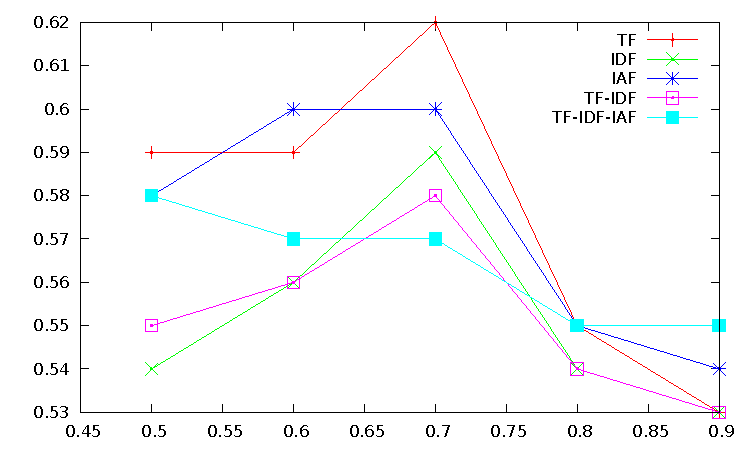
\includegraphics[width=350pt]{Figs/1-1.pdf} & 
%		\hspace{-6mm} 
		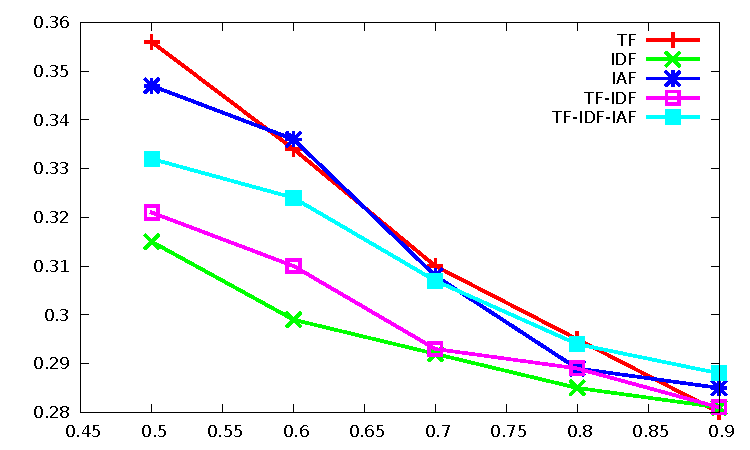
\includegraphics[width=350pt]{Figs/1-2.pdf} & 
%		\hspace{-10mm} 
		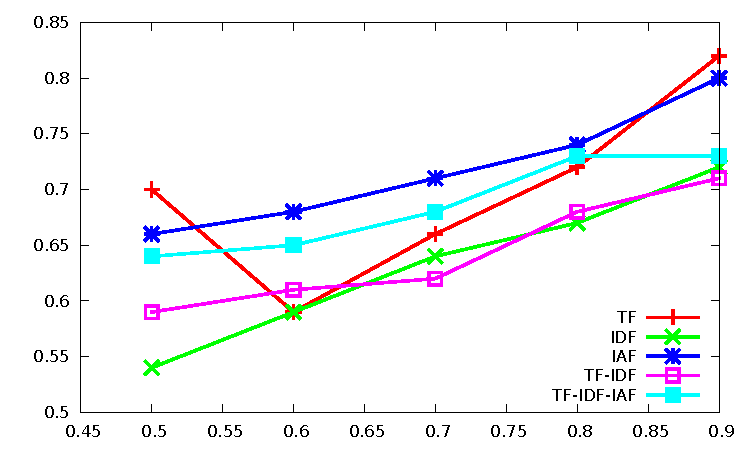
\includegraphics[width=350pt]{Figs/1-3.pdf} \\  
	
%		\vspace{4mm}
		{\LARGE Purity (Generic)} & {\LARGE NMI (Generic)} & 
		%\hspace{-3mm} 
		{\LARGE PMI (Generic)}\\
	
%		\vspace{-2mm}
%		\hspace{-8mm} 
		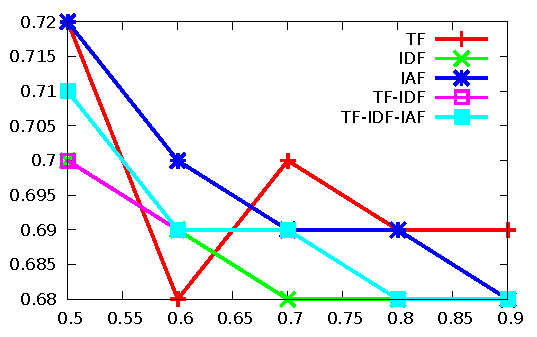
\includegraphics[width=350pt]{Figs/2-1.pdf} & 
%		\hspace{-6mm} 
		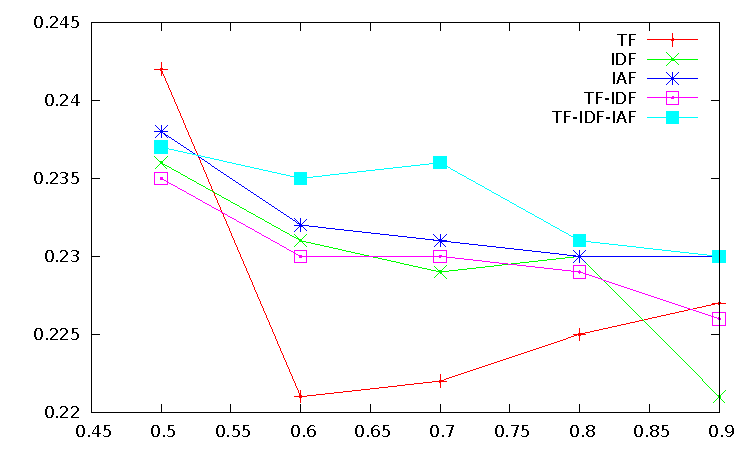
\includegraphics[width=350pt]{Figs/2-2.pdf} & 
%		\hspace{-10mm}
		 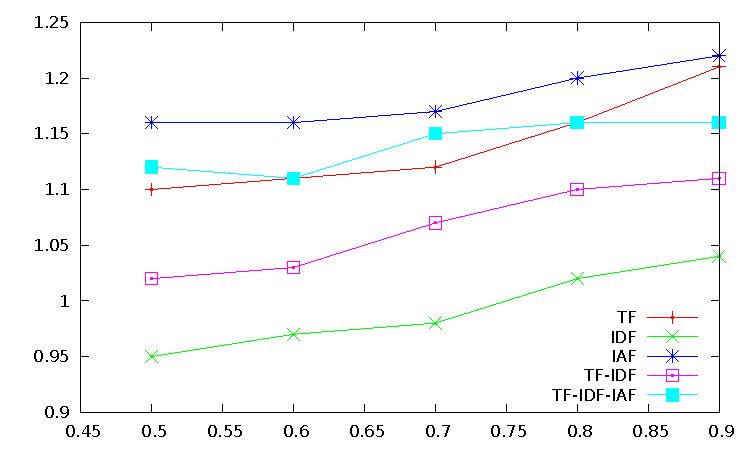
\includegraphics[width=350pt]{Figs/2-3.pdf} \\

		{\LARGE Purity (Specific)} & {\LARGE NMI (Specific)} & 
		%\hspace{-3mm} 
		{\LARGE PMI (Specific)}\\


%		\vspace{-2mm}
%		\hspace{-1mm} 
		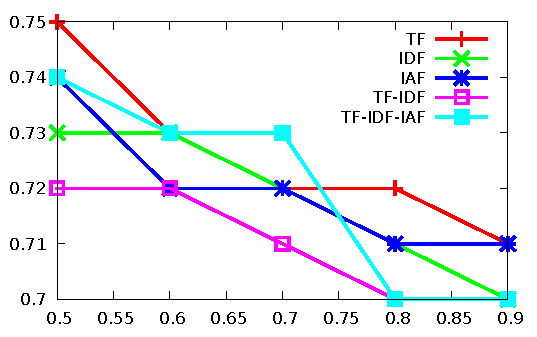
\includegraphics[width=350pt]{Figs/3-1.pdf} & 
%		\hspace{-1mm} 
		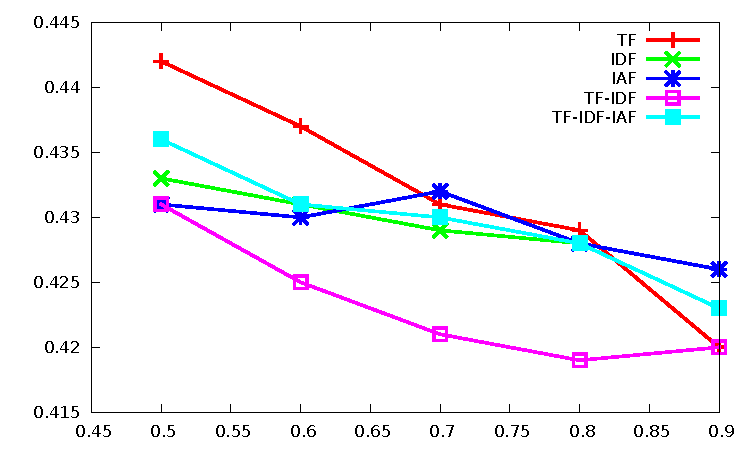
\includegraphics[width=350pt]{Figs/3-2.pdf} & 
		%\hspace{-1mm}
		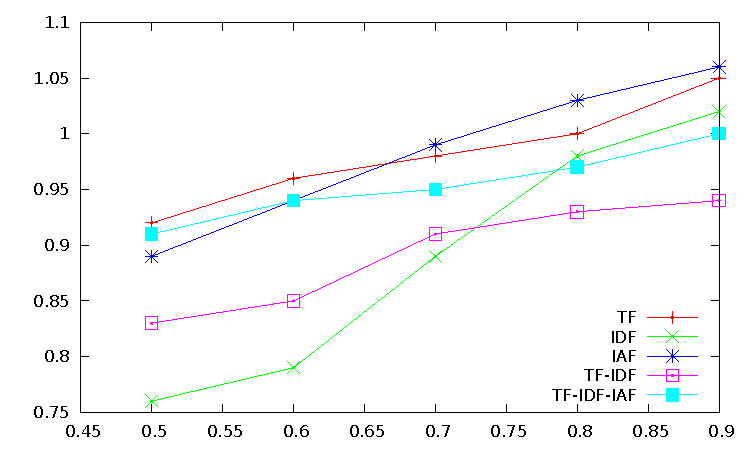
\includegraphics[width=350pt]{Figs/3-3.pdf} \\

		
%		\vspace{4mm}

		{\LARGE Purity (Events)} & {\LARGE NMI (Events)} & 
		%\hspace{-3mm} 
		{\LARGE PMI (Events)}\\

	
	\end{tabular}
}
\end{center}
\vspace{-4mm}
\caption{\footnotesize Comparison of Purity, NMI and PMI scores
  (y-axis) for five different similarity metrics (TF, IDF, IAF,
  TF-IDF, TF-IDF-IAF) for various Hashtag assignment confidence
  threshold limits (x-axis).} \label{fig-1}
\end{figure*}
%%%%%%%%%%%%%%%%%%%%%%%%%%%%%%%%%%%%%%%%%%%%%%%%%%%%%%%%%%%%%%%%%%%%%%%%%%

\section{Overall Comparison}

\label{sec:overall}

The goal of this work was to get better topics which have better
coherence without modifying the basic machinery of standard LDA. The
default way of using tweets to train LDA was to treat each tweet as a
single document (referred in this work as the Unpooled scheme). Simple
hashtag-based pooling outperformed unpooled scheme and other pooling
schemes while hashtag assignment further improved
results. Table~\ref{tbl-10} provides an overall comparison of the best
of the different schemes: Unpooled vs simple hashtag vs hashtag
assignment on the three datasets.

\begin{table}[!h]
%\setcounter{table}{13}
\centering
\resizebox{14cm}{!} 
{
	\begin{tabular}{|l|ccc|ccc|ccc|}
	\hline
	Pooling Scheme  & \multicolumn {3}{c}{Purity} & \multicolumn {3}{c}{NMI Scores} & \multicolumn {3}{c|}{PMI Scores}\\
	\hline
	 & Generic & Specific & Events &  Generic & Specific & Events &  Generic & Specific & Events\\
	\hline
	Unpooled & 0.49 & 0.64 & 0.69 & 0.29 & 0.22 & 0.39 & -1.27 & 0.47 & 0.47 \\
	\hline
	Basic Hashtagwise & 0.53 & 0.68 & 0.71 & 0.28 & 0.23 & 0.42 & 0.78 & \textbf{1.43} & \textbf{1.07} \\
	\hline
	Tag-Assignment & \textbf{0.62} & \textbf{0.72} & \textbf{0.75} & \textbf{0.36} & \textbf{0.24} & \textbf{0.44} & \textbf{0.82} & 1.21 & 1.05 \\
	\hline
	\end{tabular}
}
\caption{Overall comparison of improvement}\label{tbl-10}
\end{table}

In Table~\ref{tbl-10}, we see that the best Purity and NMI scores are
obtained by hashtag assignment while even the simple hashtag-based
pooling scheme works much better than the baseline method of unpooled
tweets. When the dataset in consideration consists of generic terms
simple hashtag pooling gives the best results in terms of topic
coherence. On the other hand when we have tweets on specific named
entities or events in general one might want to prefer hashtag
assignment as it results in best PMI scores.

\section{Related Work}

\label{sec:related_work}

Topic modeling is widely used in text mining communities with LDA
being the benchmark.  LDA has been extended in a variety of ways, and
in particular for social networks and social media, a number of
extensions to LDA have been proposed.  For example, \cite{newman11}
proposed two methods to regularize the learning of topic models aimed
at short text snippets. While the focus of this work was on blogs and
search result snippets, it would be interesting to see how well they
work on Twitter data.  Also, the combination of the work proposed in
\cite{newman11} with the tweet pooling schemes we describe before
could produce interesting results.

%There are other recent approaches for microblog retrieval, including
%estimating text quality of each tweet [ISTI-TREC2011], designing
%tweet informativeness and user/social features [Yandex-TREC2011] but
%these are not focused on improving LDA.

For automatic hashtag labeling (i.e., recommendation) that proved
crucial to improving topics in our hastag-based pooling model,
\cite{zangerle2011recommending} also uses tweet similarity as a
criteria, but does not explore metrics based on inverse author
frequency (IAF)~\cite{iaf} that we found to offer the most robust
performance across datasets and evaluation metrics.
%Moreover, the fraction of tweets with hashtags is observed as ~30+% on a large corpus, higher than what was observed on the three datasets here.


%Among the social networks, several characteristics of the data available in microblogs make them appealing for applications which fall into three broad categories: event detection [3], trend identification [4], and social group identification [5]. The interested reader is directed to the work of Liao et al[9] which discusses the opportunities and challenges related to mining microblogs.

Our work is quite different from many pioneering studies on Twitter
and topic modeling because we focus on how we could get better
topic coherence over tweets with minimal modification to existing
models. Prior work on topic modeling for tweets includes the work of
\cite{ramage} which presents a scalable implementation of a partially
supervised learning model (Labeled LDA) that maps the content of the
Twitter feed into dimensions and characterizes users and tweets using
this model. \cite{wayne} empirically compare the content of Twitter
with a traditional news medium, New York Times, using unsupervised
topic modeling. \cite{hong} use the topic modeling approach for
predicting popular Twitter messages and classifying Twitter users and
corresponding messages into topical categories.

The {T}witterRank system~\cite{Weng2010wsdm} and \cite{hong} uses
author-based pooling to apply LDA to tweets. \cite{wayne} compared
topic characteristics between twitter and traditional news media (NY
Times); they propose to use one topic per tweet (in a manner similar to
PLSA), and argues (with some evidence) that this is better than no
pooling, or the author-topic model. \cite{kireyev2009} used term weighting
to tackle term sparseness in LDA, the weights are derived from LSA
vector length. \cite{Naveed2011cikm} used LDA for tweet retrieval. In
addition, they used retweet as an indicator of "interestingness" to
improve retrieval quality, which suggests additional features we
could incorporate in future extensions to our pooling framework.

Our work is different from these in the sense that we provide a simple
yet effective way which greatly improves the quality of topics
obtained without making any major complicated modifications to
standard LDA. The detailed experiments on a variety of datasets
highlight our novel contribution of hashtag-based pooling and automatic
hashtag labeling using similarity metrics like IAF~\cite{iaf} as an
approach that improves a range of topic coherence measures.

%Evaluating topic models has continued to be an active research topic
%with the aim of automatically evaluating topic models. Newman et l
%[10] introduce the task of topic coherence evaluation, whereby a set
%of words, as generated by a topic model, is rated for coherence or
%interpretability. Wallach [11] present evaluation methods based on
%the probability of held-out documents given a trained model.

\section{Summary and Conclusion}

\label{sec:conclusion}

The work described in this paper presents a way of aggregating tweets
in order to improve performance of topic models in terms of quality of
topics obtained measures by the ability to reconstruct clusters and
topic coherence. The initial results presented in Table~\ref{tbl-456}
suggest that hashtag-based pooling outperforms all other pooling
strategies including the default way of training topic models on
Twitter data(unpooled).

Since a major portion of Twitter data does not contains hashtags we
looked at ways of assigning hashtags to tweets. Insights from Hashtag
Assignment results (Table~\ref{tbl-9}) suggest that when the main aim
is to use the topics obtained to extract different events mentioned in
the Twitter data one should use hashtag assignment with a relaxed
threshold(~0.5). The high values of Purity scores and NMI values for
low threshold support this claim.

When the goal is to obtain interesting topics with topic words
pertaining to the same common theme (coherent topic words), hashtag
assignment with strict constraints (a threshold of $\sim 0.9$) works
well. The PMI scores in Table~\ref{tbl-9} highlight that topic
coherence increases as we move down the column. Thus the threshold of
0.9 gives most coherent topics.

Overall, results shown in Table~\ref{tbl-10} compare unpooled scheme
with simple hashtag pooling and hashtag assignment schemes.  In short,
across all datasets and metrics, the best hashtag assignment method
performs optimally or near-optimally indicating the promise of this
novel automatic hashtag labeling and pooling approach.

To this end, we have achieved our initial goal.  We have introduced
novel techniques for automatic tweet hashtag labeling and pooling that
have produced topics representative of the events queried to construct
the source data and have substantially improved various quantitative
measures of topic coherence.  Further, we have achieved this without
modifying the LDA algorithm itself but rather by preprocessing its
input.

This technique worked well across a diverse set of data and suggests
that continued investigation into aggregation techniques for topic
modeling on short text and microblog documents is warranted given its
highly successful outcome demonstrated in this work.

%\section*{Acknowledgments} 
%
%NICTA is funded by the Australian
%Government as represented by the Department of Broadband,
%Communications and the Digital Economy and the Australian Research
%Council through the ICT Centre of Excellence program.

%'apalike-fr' style below applies smallcaps style on author names
%in order to apply 'apalike-fr' the babel package must be given [frenchb] option instead of [english]
% \usepackage[frenchb]{babel} also causes title "References" to render with French accents like "R\'ef\'erences"
%\bibliographystyle{apalike-fr}

%'apa' style does not apply "smallcaps style" on author names and goes with the [english] option in the babel package

%\bibliography{colingbiblio}
%\bibliographystyle{apa}

\bibliographystyle{apa}
\bibliography{colingbiblio}
% \nocite{*}
%\bibliographystyle{coling2012

%\nocite{TALN2007,LaigneletRioult09,LanglaisPatry07,au1972,cks1981,mb2012}

%%================================================================
\end{document}


Latent Dirichlet allocation (LDA) \cite{blei03} is a generative model for text. In LDA, each document may be viewed as a mixture of various topics. We use the following notations for describing the LDA model:\\
\hspace{2cm} M : number of documents\\
\hspace{2cm} N : number of words in a document\\
\hspace{2cm} $\alpha$ : parameter of the Dirichlet prior on the per-document topic   distributions\\
\hspace{2cm} $\beta$ : the parameter of the Dirichlet prior on the per-topic word distribution\\
\hspace{2cm} $\theta_i$ : the topic distribution for document i,\\
\hspace{2cm} $\phi_k$ is the word distribution for topic k,\\
\hspace{2cm} $z_{ik}$ is the topic for the jth word in document i, and\\
\hspace{2cm} $w_{ij}$ is the specific word.
 
The $w_{ij}$ are the only observable variables, and the other variables are latent variables. If K be the number of topics considered in the model, $\phi$ is a $K*V$ (V is the dimension of the vocabulary) matrix each row of which denotes the word distribution of a topic.

The generative process behind is that documents are represented as random mixtures over latent topics, where each topic is characterized by a distribution over words. LDA assumes the following generative process for each document i in a corpus D :

\begin{compactenum}
\item Choose $\phi_i \sim Dir(\alpha)$, where i $\in$ {1,...,M} and Dir($\alpha$) is the Dirichlet distribution for parameter $\alpha$
\item Chose $\phi_k \sim Dir(\beta)$, where k $\in {1,...,K}$
\item For each of the words $w_{ij}$, where j $\in {1,...,N_i}$
	\begin{compactenum}
		\item Chose a topic $z_{i,j} \sim Multinomial(\theta)$
		\item Chose a word $w_{i,j} \sim Multinomial(\phi_{z_{i,j}})$
	\end{compactenum}
\end{compactenum}


Learning the various distributions (the set of topics, their associated word probabilities, the topic of each word, and the particular topic mixture of each document) is a problem of Bayesian inference. The original paper used a variational Bayes approximation of the posterior distribution; alternative inference techniques use Gibbs sampling and expectation propagation.







%In this model, a “topic” t is a discrete distribution over words with probability vector $\phi_{t}$. Dirichlet priors, with concentration parameter $\beta$ and base measure $n$, are placed over the topics $\Phi = \lbrace \phi_{1}, ... , \phi_{T} \rbrace $ :

%\begin{center}
%$P\left( \Phi \right)  = \Pi_{t}  Dir\left(  \phi_{t} ; \beta n  \right) $
%\end{center}

%Each document, indexed by d, is assumed to have its own distribution over topics given by probabilities $\theta_{d}$. The priors over $\Theta = \lbrace  \theta_{1}, ... , \theta_{d}  \rbrace$ are also Dirichlet, with concentration parameter $\alpha$ and base measure $m$:

%\begin{center}
%$P\left( \Theta \right)  = \Pi_{d}  Dir\left(  \theta_{d} ; \alpha m  \right) $
%\end{center}

%The tokens in a document $w^{d} = \lbrace w^{d}_{n} \rbrace^{N_{d}}_{n=1} $ (where $N_d$ is the number of tokens in the document d)are associated with topic assignments $z^{d} = \lbrace z^{d}_{n} \rbrace^{N_{d}}_{n=1} $, drawn i.i.d. from the document-specific topic distribution:
%\begin{center}
%$P\left( z_{d} | \theta_{d}  \right) = \Pi_{n} \theta_{ z^{\left( d\right) }_{n} %| d}$.
%\end{center}
%The tokens are drawn from the topics’ distributions:
%\begin{center}
%$P\left( w_{d} | z_{d}, \Phi  \right) = \Pi_{n} \phi_{ w^{\left( d\right) }_{n} | z^{\left( d\right) }_{n}}$.
%\end{center}

%A data set of documents $W = \lbrace w^(1) , w^(2) , ..., w^(D) \rbrace $ is observed, while the underlying corresponding topic assignments $Z = \lbrace z^(1) , z^(2) , ..., z^(D) \rbrace $ are unobserved. 
%\\



\begin{table}[!h]
%\setcounter{table}{4}
\centering
%\resizebox{14cm}{!} 
%{
	\begin{tabular}{|l|c|c|c|c|c|}
	\hline
	Pooling Scheme & Unpooled & Author & Hourly & Burstwise & Hashtag\\
	\hline
	Generic & 0.49 & \textbf{0.54} & 0.45 & 0.42 & \textbf{0.54}\\
	\hline
	Specific & 0.64 & 0.62 & 0.61 & 0.60 & \textbf{0.68}\\
	\hline
	Events & 0.69 & 0.70 & 0.61 & 0.64 & \textbf{0.71} \\
	\hline
	\end{tabular}
%}
\caption{Purity Scores for different datasets}\label{tbl-4}
\end{table}


\begin{table}[!h]
%\setcounter{table}{5}
\centering
%\resizebox{14cm}{!} 
%{
	\begin{tabular}{|l|c|c|c|c|c|}
	\hline
	Pooling Scheme & Unpooled & Author & Hourly & Burstwise & Hashtag\\
	\hline
	Generic & 0.28 & 0.24 & 0.07 & 0.18 & \textbf{0.28}\\
	\hline
	Specific & 0.22 & 0.17 & 0.09 & 0.16 & \textbf{0.23}\\
	\hline
	Events & 0.39 & 0.41 & 0.32 & 0.33 & \textbf{0.42}\\
	\hline
	\end{tabular}\caption{NMI Scores for different datasets}\label{tbl-5}
%}
\end{table}


\begin{table}[!h]
%\setcounter{table}{6}
\centering
%\resizebox{14cm}{!}
%{
	\begin{tabular}{|l|c|c|c|c|c|}
	\hline
	Pooling Scheme & Unpooled & Author & Hourly & Burstwise & Hashtag\\
	\hline
	Generic & -1.27 & 0.21 & -1.31 & 0.48 & \textbf{0.78}\\
	\hline
	Specific & 0.47 & 0.79 & 0.87 & 0.74 & \textbf{1.43}\\
	\hline
	Events & 0.47 & 0.51 & 0.22 & 0.58 & \textbf{1.07}\\
	\hline
	\end{tabular}\caption{PMI Scores for different datasets}\label{tbl-6}
%}
\end{table}
